\documentclass[a4paper]{article}
\usepackage{amsmath,amssymb,caption,float,graphicx,tabularx,xcolor}
\captionsetup[table]{labelsep=period}
% \renewcommand\thesection{\arabic{section}}
\begin{document}
\begin{center}
    \huge
    \textbf{ECE4810J\\System-on-Chip Design\\}
    \Large
    \vspace{15pt}
    \uppercase{\textbf{Lab 0}}\\
    \large
    \vspace{5pt}\today\\
    \vspace{5pt}
    Yihua Liu 518021910998
    \vspace{5pt}
    \rule[-5pt]{.97\linewidth}{0.05em}
\end{center}
1. (10\%) What are the benefits of having Programmable logic on Zynq?

Programmable logic offers an ideal resource for implementing algorithms inherently parallel in nature; for example in signal and image processing, where mathematical operations are performed on a large number of samples or pixels simultaneously. Besides, the Zynq PL has the ability to easily instantiate multiple IP blocks which can act as AXI masters.
It can couple with the processor (PS) to allow the differing properties of these two resources to be maximally exploited when partitioning the system into software and hardware elements. It provides a perfect platform in which to create co-processing cores due to the ability to perform parallel execution.\\
2. (20\%) How many cores does Zynq-7000 have? What are the names of those cores? How does the memory hierarchy look like? What is the main CPU frequency?

Zynq-700 has 2 cores. Those cores are ARM Cortex-A9 with NEON and FPU extensions. The memory hierarchy consists of DDR memory, I-cache, D-cache, and processor cache: Dynamic RAM (DRAM), Static RAM (SRAM), Level 1 (L1) Cache, Level 2 (L2) Cache, Level (L3) Cache.

Main CPU frequency for Z-7010, Z-7015, and Z-7020 (the PS on the Artix-7 based devices) is 866 MHz, and 1 GHz for Z-7030, Z-7045, and Z-7100 (the Kintex-based devices) (processor type: ARM Cortex-A9). Arty Z7 integrating ARM Cortex-A9 processor has a CPU frequency of 650 MHz.
\begin{figure}[H]
    \centering
    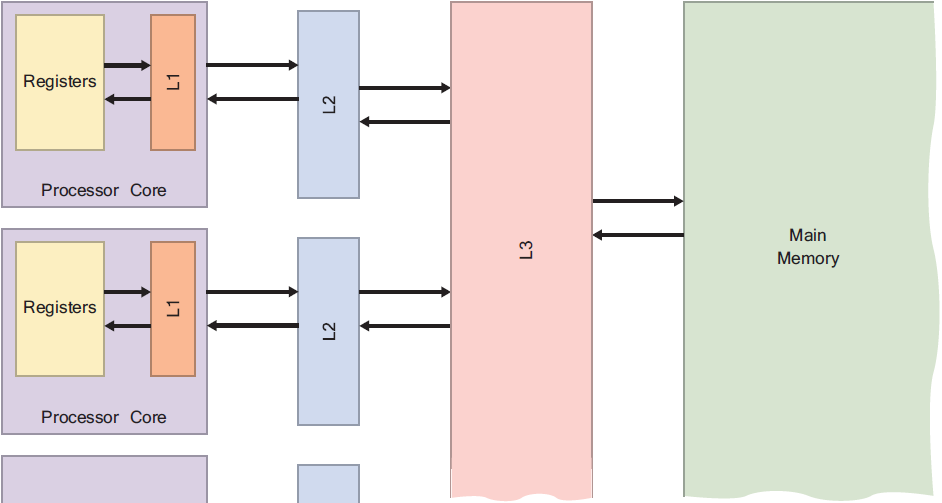
\includegraphics[width=1\textwidth]{1.png}
    \caption{Cache levels and their locations relative to the processor cores and main memory.}
\end{figure}
3. (15\%) Please list the main interfaces of the Zynq-7000 AP SoC device.\\
PS-PL AXI Interfaces: M\_AXI\_GP0, M\_AXI\_GP1, S\_AXI\_GP0, S\_AXI\_GP1, S\_AXI\_ACP, S\_AXI\_HP0, S\_AXI\_HP1, S\_AXI\_HP2, S\_AXI\_HP3.\\
PL Co-Processing Interfaces: Accelerator Coherency Port (ACP) Interface.\\
Interrupt Interfaces.\\
Memory Interfaces: 1. Dynamic Memory Interface; 2. Static Memory Interface: NAND flash, Parallel (SRAM/NOR).\\
Programmers model interface to the GIC, Distributor and CPU interfaces.\\
4. (5\%) How is the Arty Z7 board powered?

It is powered from USB or any 7V-15V external power source. It is powered from the Digilent USB-JTAG-UART port (J14) or from some other type of power source such as a battery or external power supply. An external power supply (e.g. wall wart) can be used by plugging it into the power jack (J18) and setting jumper JP5 to “REG”. Similar to using an external power supply, a battery can be used to power the Arty Z7 by attaching it to the shield connector and setting jumper JP5 to “REG”.
\begin{table}[H]
    \centering
    \begin{tabular}{|c|c|c|}
        \hline
        Supply&Circuits&Current (max/typical)\\
        \hline
        3.3V&FPGA I/O, USB ports, Clocks, Ethernet, SD slot, Flash, HDMI&1.6A/0.1A to 1.5A\\
        \hline
        1.0V&FPGA, Ethernet Core&2.6A/0.2A to 2.1A\\
        \hline
        1.5V&DDR3&1.8A/0.1A to 1.2A\\
        \hline
        1.8V&FPGA Auxiliary, Ethernet I/O, USB Controller&1.8A/0.1A to 0.6A\\
        \hline
    \end{tabular}
    \caption{Arty Z7 power supplies.}
\end{table}
5. (10\%) What is the Quad SPI Flash? What is the usage of it on this board?

Quad SPI Flash, i.e., Quad SPI serial NOR flash, is a Multi-I/O SPI Flash memory that is used to provide non-volatile code and data storage and initialize the PS subsystem as well as configure the PL subsystem.\\
6. (10\%) What is DDR Memory? What is the usage of it?

DDR Memory, i.e., the multi-protocol Double Data Rate memory controller, consists of three major modules: a core memory controller and scheduler (DDRC), an AXI memory port interface (DDRI) and a digital PHY and controller (DDRP). It can be configured to operate in either 16-bit or 32-bit mode, offering access to a 1 GB address space with a single rank DRAM memory configuration of 8-, 16- or 32-bit.\\
7. (20\%) What are the main custom IP blocks creation methods Xilinx provides?
Implemented in the PL:
\begin{itemize}
    \item The Xilinx library
    \item Third Party sources
    \item Designed by the User, or by colleagues within the same organisation (‘in-house’)
\end{itemize}
IP Core Design Methods/IP Creation Method (tools which enable the creation of custom IP blocks for use in your own embedded system designs):
\begin{itemize}
    \item HDL (Hardware description languages, such as VHDL and Verilog)
    \item System Generator
    \item HDL Coder (MathWorks HDL Coder)
    \item Vivado High-Level Synthesis: IP-XACT, IP Core, SysGen (Xilinx Vivado HLS)
\end{itemize}
8. (10\%) What is High-Level Synthesis (HLS)? What are the motivations behind HLS?

High-level synthesis means synthesising the high-level C, C++ or SystemC code into an HDL description, which would thereafter undergo logic synthesis to obtain a netlist. Here, ‘synthesis’ refers to logic synthesis, i.e. the process of analysing and interpreting HDL code and forming a corresponding netlist.

Motivation: 'productivity'
\begin{itemize}
    \item With a high-level representation abstracting low-level detail, the implication is that the description of the circuit becomes simpler. The result is that designs can be generated much more rapidly than using more traditional methods. Variations on the architecture can be created quickly by applying appropriate directives to the HLS process.
    \item High-level synthesis from software languages is convenient for many designers, as these languages are widely adopted for developing algorithms and system-level descriptions. The facility to rapidly convert from software to hardware design languages therefore constitutes a simplification of the design process.
    \item HLS is also beneficial in terms of systems development and software/hardware partitioning, as there is a common language for targeting both elements of the system; this makes it easy to adapt and retarget parts of the design as it is iterated to completion.
\end{itemize}
\end{document}